\chapter{Family Connection: A Guide to Lightspan}

\begin{figure}[H]
    \centering
    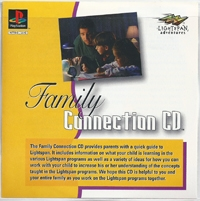
\includegraphics[width=0.5\textwidth]{"./Games/FamilyConnection/Images/FamilyConnectionAGuidetoLightspanCDCover.jpg"}
    \caption{Family Connection: A Guide to Lightspan - CD Cover}
\end{figure}

Family Connection: A Guide to Lightspan was a promotional CD that was produced by The Lightspan Partnership in order to showcase and highlight the importance of integrating technology with education.

The "game" itself, similar to 16 Tales, is split into three sections:

\begin{itemize}
    \item Introducing The Lightspan Partnership
    \item Powerful Learning Programs
    \item Lightspan Adventures
\end{itemize}

Introducing The Lightspan Partnership and Powerful Learning programs are individuals videos on their own.
Lightspan Adventures, on the other hand, is split into three separate videos detailing  the three age groups that Lightspan catered to:

\begin{itemize}
    \item Grades K-2
    \item Grades 3 \& 6
    \item Grades 5 \& 6
\end{itemize}

Each of the Lightspan Adventure series of videos also includes a selection of additional videos highlighting a number of the games which they have on offer.

The combined runtime of all the videos on this CD is just under an hour.

\newpage

\section{List of screenshots:}

\begin{figure}[H]
    \centering
    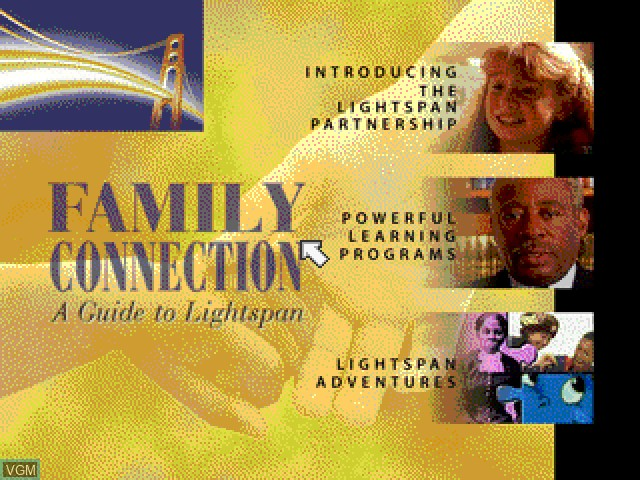
\includegraphics[width=0.5\textwidth]{"./Games/FamilyConnection/Images/FamilyConnectionAGuidetoLightspanMainMenu.jpg"}
    \caption{Screenshot of the main menu}
\end{figure}

\begin{figure}[H]
    \centering
    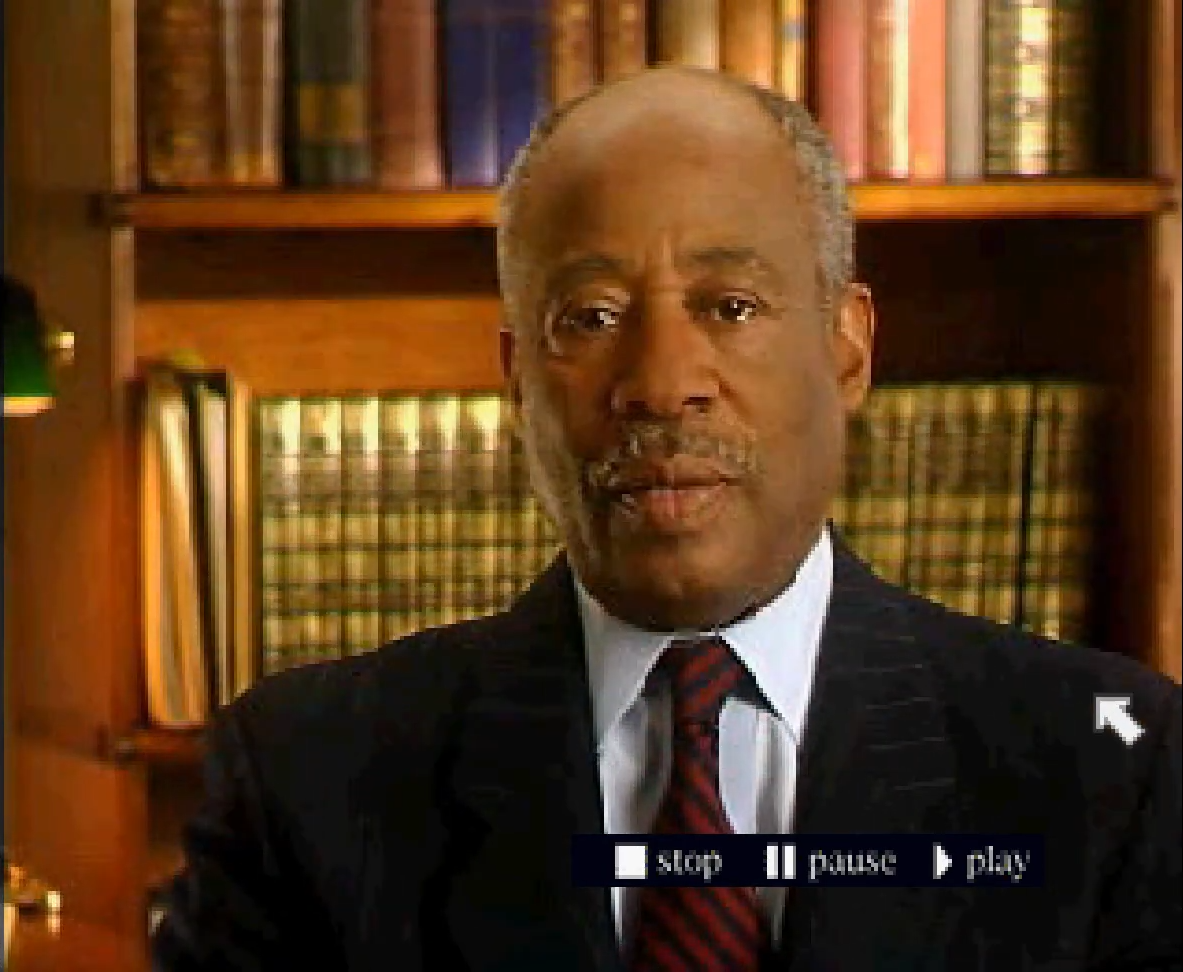
\includegraphics[width=0.5\textwidth]{"./Games/FamilyConnection/Images/FamilyConnectionAGuidetoLightspanScreenshot1.png"}
    \caption{Screenshot taken from the video "Powerful Learning Programs"}
\end{figure}

\begin{figure}[H]
    \centering
    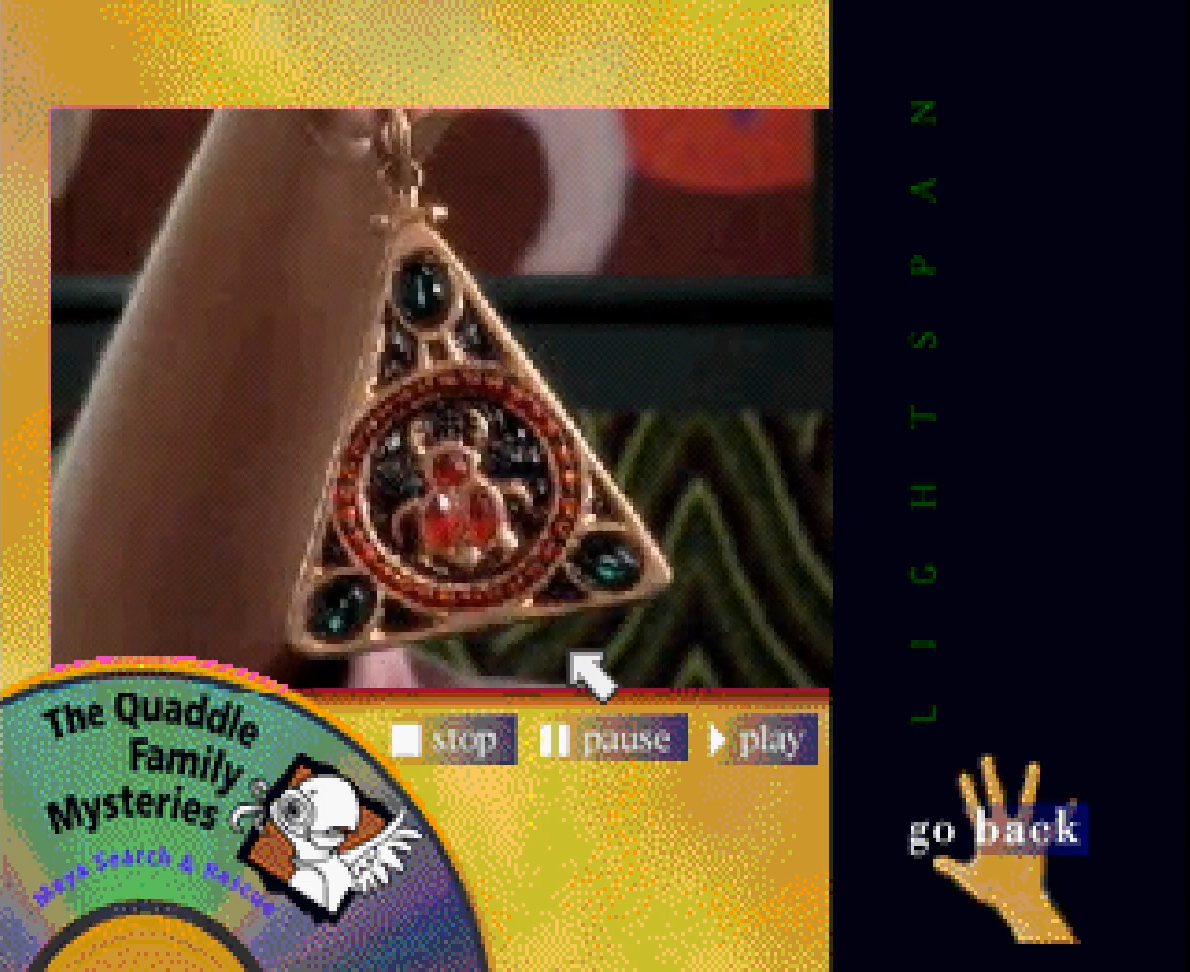
\includegraphics[width=0.5\textwidth]{"./Games/FamilyConnection/Images/FamilyConnectionAGuidetoLightspanScreenshot2.png"}
    \caption{Screenshot from one of the Lightspan Adventures videos}
\end{figure}

\clearpage
\newpage

\section{Main Menu audio transcription}

Welcome to the Family Connection.
We hope this guide to Lightspan will be helpful as you and your family discover new learning opportunities.
Simply click on any of the three pictures to start exploring.

\section{Introducing The Lightspan Partnership audio transcription}

Schools today are surrounded by change - the communities we serve, the kinds of challenges kids face, the demands of the working world have all changed tremendously since I first started teaching.

But one thing will never change - we educators will always have to prepare kids to thrive.
If we're going to keep living up to that responsibility, I think we need to change too.
We have to take the best of what we've always done, reinvent it and make it better. We have to find new tools and new ways of doing things.

The Lightspan Partnership is working with teachers, families, and students to meet today's educational challenges.
We're creating powerful tools that motivate and help children to learn - tools that expand learning in schools and homes, tools that will prepare our children for the challenges of tomorrow.

"Watch what happens when we increase the gravity by just five percent."

"Good, now why do you think that happens?"

There's a natural love of learning in every young child. Our challenge is teachers is to find ways each day to engage that part of them, to nourish it, to focus it on meaningful work so that it keeps growing for a lifetime.

Knowledge and skill grow with practice - learning an idea and then applying it, thinking critically, experimenting, solving problems.
You have to give kids lots of ways to do that.
She can't do it all with a chalkboard.

Kids love great characters and interesting stories.
Who doesn't?
But we need to see more of the time kids spent on entertainment spent on learning.
What if the same people who make the best movies and games would help us educators make things that teach?
Then kids would run home from school and keep on learning whether we told them to or not.
Now that would be a big help.

Teachers and families need to work together to meet the needs of every child.
When parents can see what their children are doing every day, it's easier for them to work together as partners.

"So what did you do in school today?"

"I adjusted my angle by 16 degrees, see, so I would have hit the meteor."

"Oh so look out, look out! So you use geometry to figure out how the rock misses the ship?"

"Yeah!"

"Hey Nick, you did a great job on your history project."

"Thanks, you want to check out Family Activities?"

"Okay."

In sixth grade reading, your child will find more subject material in history and current events.

Powerful educational programming created by some of our finest educators.
Motivating tools designed to challenge and inspire.
An expanded partnership between teachers, students, and families.
This is the Lightspan Partnership.

\section{Powerful Learning Programs audio transcription}

Growing up, I was lucky enough to go to an excellent school with wonderful teachers and to get a terrific education.
And I've devoted most of my life to education as a teacher, counselor, principal, and superintendent.
I was academic vice president at Temple University and was appointed by three presidents - Lyndon Johnson, Jimmy Carter, and Bill Clinton - to national advisory councils on education.

When I went to school, and even when I started teaching, the teacher stood in front of a class while students listened and took notes.
And in most places, that's how teaching is still being done because, for the most part, it works pretty well.
But today there's also an opportunity to use technology to present some of these same ideas and information in ways that I never could with a textbook or a chalkboard - ways that really bring concepts to life and get kids excited about learning.

The Lightspan partnership is working with teachers, families, and students using some of this new technology to develop learning tools that are truly powerful.
The main objective of these programs is to help children learn, so the Lightspan programs start with solid educational content.
They are developed to match the textbooks and other curriculum currently used in your child's classroom, so your child's teacher can easily integrate them into his or her current instruction plans.
And they are developed by expert teachers who have years of successful experience in the classroom.

The focus of these programs is on reading, language arts, and mathematics - the basic skills that we all know are so important for future success.
One of the most important aspects of these programs is that they are flexible and can be tailored to meet the needs of your child.

The Lightspan programs not only teach our children, but they also do so in a way that's motivating, so kids will want to spend time learning because these programs are as much fun and are as exciting as all the other activities that kids enjoy.
And by repeating an activity, they'll master the educational concept, and they'll retain it.
And we all know nothing builds self-confidence and motivation more than success - that sense of accomplishment when we did something that we didn't think we could do.

And for families, Lightspan provides a tremendous opportunity to enhance what children are learning in the classroom by continuing that learning at home.
Parents can see what their child is doing in school, and families can work together with this technology in their own living room whenever they have time.
Lightspan also provides lots of ideas and suggestions for fun, rewarding activities that you can do with your child.

As you work with these programs and see for yourself how your child reacts to them, I am confident that you will see these programs are truly powerful and open up tremendous opportunities for the education of our children.

\section{Lightspan Adventures: Grades K-2 audio transcription}

"My children really love Lightspan.
They love the songs, they love the characters.
They liked interacting with the characters and with the the challenge of it."

"The Lightspan programs teach vocabulary, they teach reading, they teach math in a variety of different ways."

"Blue hat, four-sided head, triangular nose, shiny shoes - that's him."

"And it's very nice because the parent and the child can sit down and work on it together, and they're both involved.
And I think it's just a good way for parents and and children to work together and be working on some of being academic but in a more fun type of way."

"We had an open house, and the first thing the students wanted to show the parents was Lightspan."

"Why don't you tell me what's happening?"

"Okay?"

"And it was so wonderful to see the students showing the parents how they could use it, how they were reading, how they were doing math skills.
And it was wonderful."

\section{Lightspan Adventures: Grades 3 \& 4 audio transcription}

"Lightspan corresponds perfectly with the curriculum that we're using today.
It goes along with all of the books that we're using, all of the programs that provide us with information on prefixes and suffixes - everything.
Lightspan helps to bridge the connection between the home and the teacher and the child"

"I think Lightspan has encouraged parents and teachers to work together because there's a common thread now, both at school and at home."

"The kids can't wait to get on Lightspan, and sometimes I have to hold them back."

"I think Lightspan has been a giant step, bringing technology into the classrooms."

\section{Lightspan Adventures: Grades 5 \& 6 audio transcription}

"My students really enjoy Lightspan.
It's very appealing to them.
They like the graphics, they like the storyline.
It's very age appropriate for them.
They choose to do it when they have free time, spare time."

"When the Lightspan program stratus goes into the home, with parents and students working together, I see that there's going to be a lot of communication happening between parent and child, as well as problem solving."

"So what did you do in school today?"

"I adjusted my angle by 60°."

"The Lightspan concept of parents and families and teachers and students all working together is a very, very important one."

"You want to check out Family Activities?"

"Okay."

"If students are using the Lightspan program at home with their parents, they'll be actually reading more.
They're also learning about characters in history, they're problem solving, they're learning vocabulary.
So this can only benefit their education."